\documentclass{beamer}

\usepackage[utf8]{inputenc}
\usepackage{hyperref}

\usetheme{Berkeley}
\beamertemplatenavigationsymbolsempty
\setbeamertemplate{headline}{}
 
\title{Import FoodChain-Lab Workflow}
\date{}
 
\begin{document}
\maketitle
 
\section{1}
\begin{frame}
	\begin{center}
  		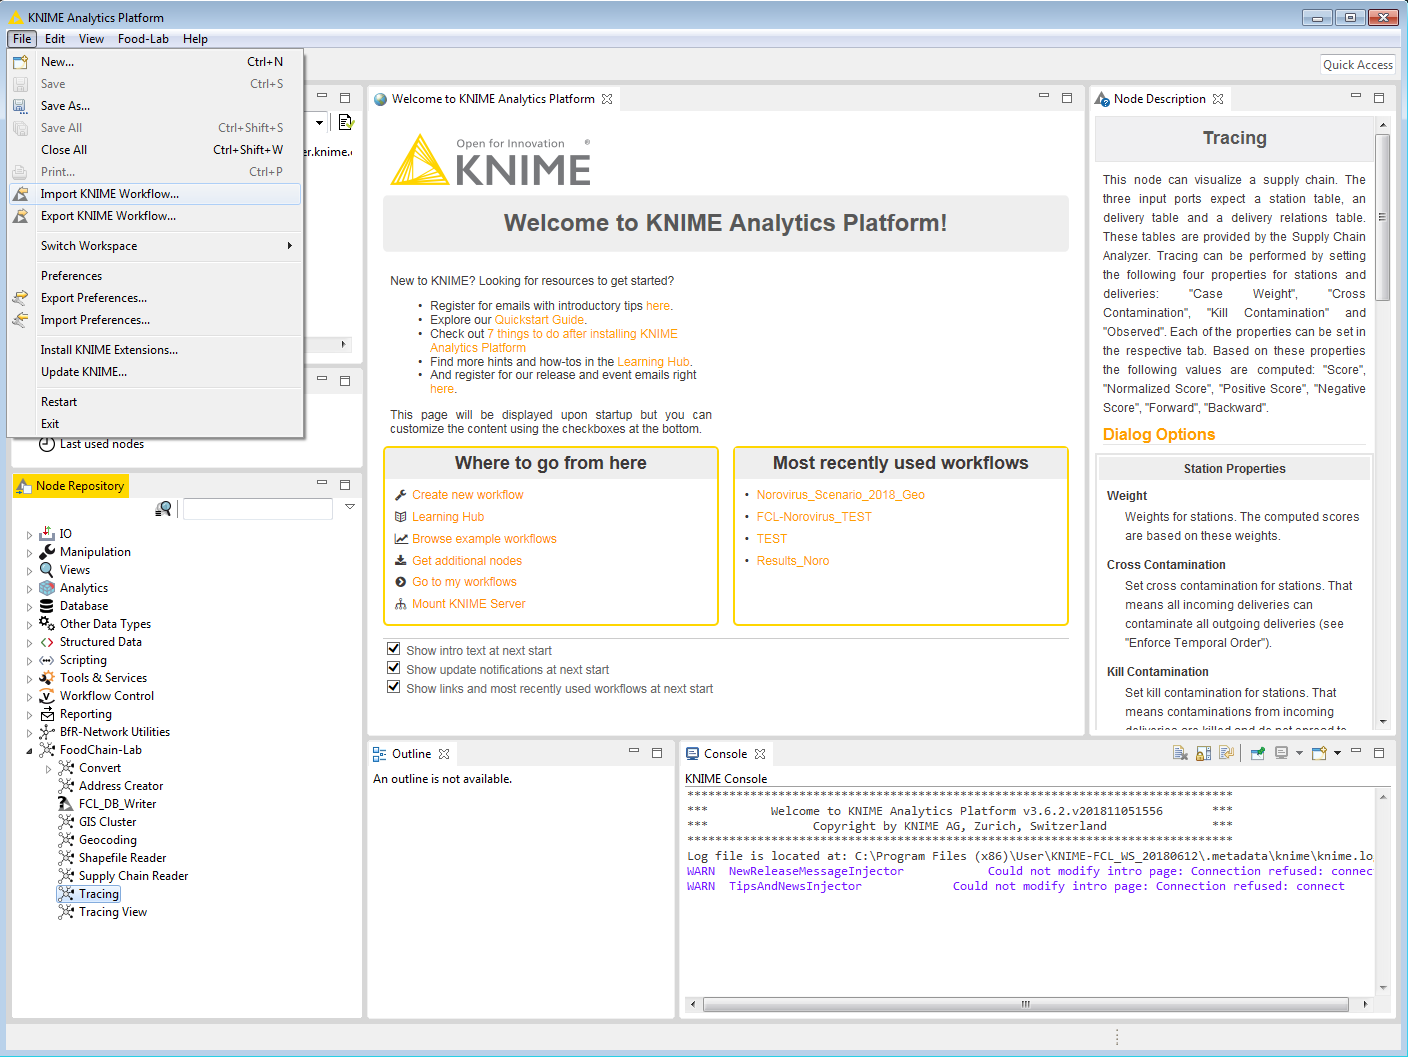
\includegraphics[height=0.6\textheight]{1.png}
	\end{center}
	\begin{itemize}
		\item Download Example Workflow: \url{https://github.com/SiLeBAT/BfROpenLabResources/raw/master/GitHubPages/workflows/FCL_Example.zip}
		\item Right click on \textbf{LOCAL} in the \textbf{KNIME Explorer} view and select \textbf{Import KNIME Workflow}.
	\end{itemize}
\end{frame}

\section{2}
\begin{frame}
	\begin{center}
  		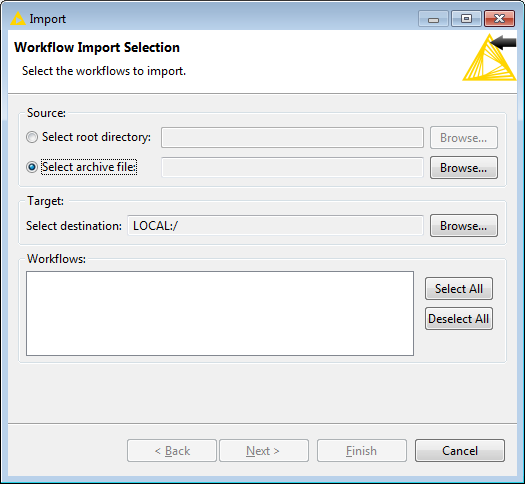
\includegraphics[height=0.6\textheight]{2.png}
	\end{center}
	\begin{itemize}
		\item In the Import dialog that appears, select \textbf{Select archive file} and click the \textbf{Browse} button to the right of it.
	\end{itemize}
\end{frame}

\section{3}
\begin{frame}
	\begin{center}
  		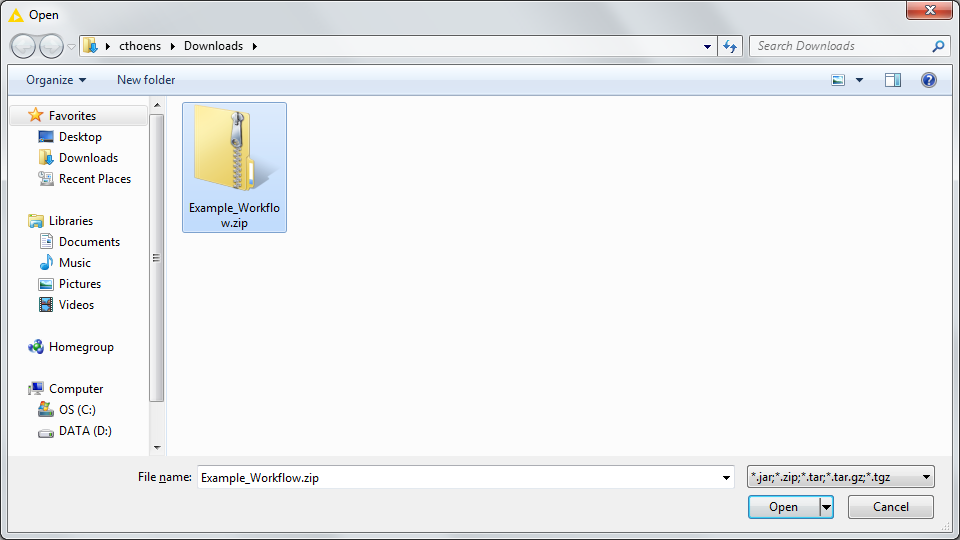
\includegraphics[height=0.6\textheight]{3.png}
	\end{center}
	\begin{itemize}
		\item In the Open dialog that appears, select the downloaded zipped workflow and Click \textbf{Open}.
	\end{itemize}
\end{frame}

\section{4}
\begin{frame}
	\begin{center}
  		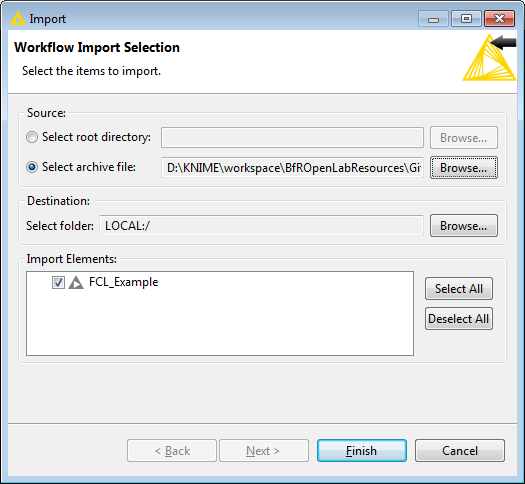
\includegraphics[height=0.6\textheight]{4.png}
	\end{center}
	\begin{itemize}
		\item In the Import dialog, you'll see the selected workflow.
		\item Click \textbf{Finish}.
	\end{itemize}
\end{frame}

\section{5}
\begin{frame}
	\begin{center}
  		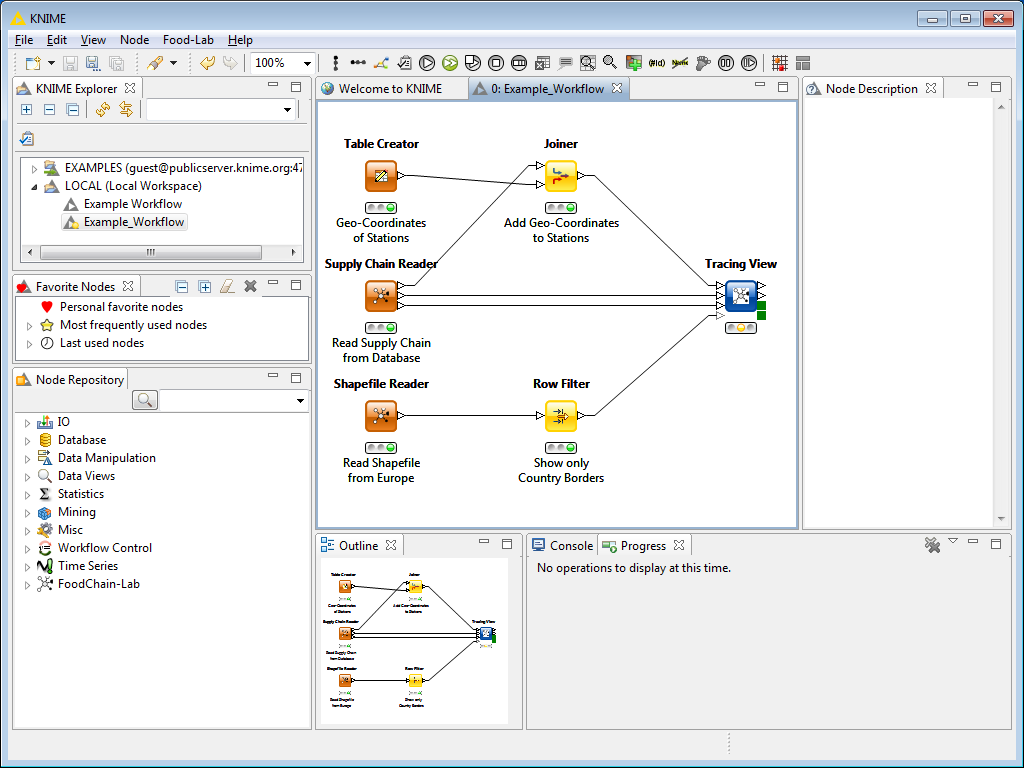
\includegraphics[height=0.6\textheight]{5.png}
	\end{center}
	\begin{itemize}
		\item In the KNIME workbench, expand \textbf{LOCAL} in the \textbf{KNIME Explorer} view and double click on the imported workflow.
		\item The workflow should show up in the Workflow Editor now.
	\end{itemize}
\end{frame}

\end{document}